\usetikzlibrary{arrows.meta,calc}
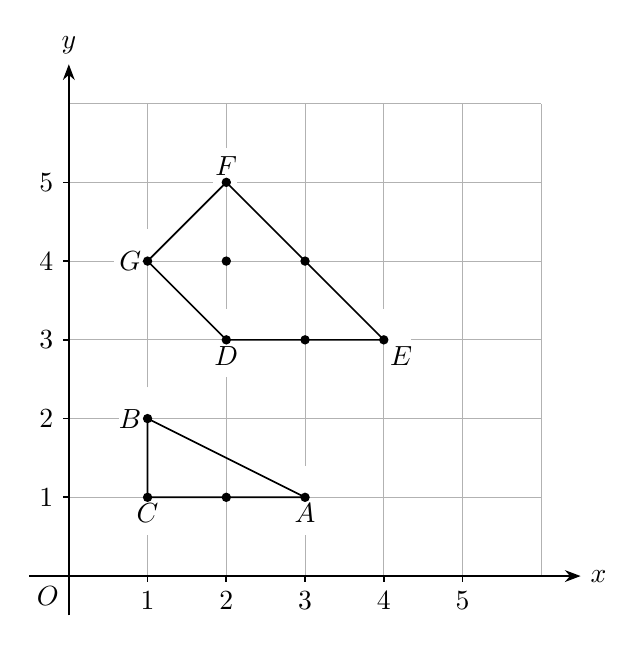
\begin{tikzpicture}[x=1cm,y=1cm,line width=.6pt,font=\normalsize,>=Stealth]
\draw[gray!60,line width=.3pt] (1.0000000000,0.0000000000)--(1.0000000000,0.5213388528);
\draw[gray!60,line width=.3pt] (1.0000000000,0.9930917486)--(1.0000000000,1.0408336137);
\draw[gray!60,line width=.3pt] (1.0000000000,1.4093125944)--(1.0000000000,2.0408597438);
\draw[gray!60,line width=.3pt] (1.0000000000,2.3962643847)--(1.0000000000,4.0408911266);
\draw[gray!60,line width=.3pt] (1.0000000000,4.4093701073)--(1.0000000000,6.0000000000);
\draw[gray!60,line width=.3pt] (0.0000000000,1.0000000000)--(6.0000000000,1.0000000000);
\draw[gray!60,line width=.3pt] (2.0000000000,0.0000000000)--(2.0000000000,2.5268452072);
\draw[gray!60,line width=.3pt] (2.0000000000,2.9985981030)--(2.0000000000,3.0408789147);
\draw[gray!60,line width=.3pt] (2.0000000000,3.3962835557)--(2.0000000000,4.9639396667);
\draw[gray!60,line width=.3pt] (2.0000000000,5.4356925625)--(2.0000000000,6.0000000000);
\draw[gray!60,line width=.3pt] (0.0000000000,2.0000000000)--(0.6343828286,2.0000000000);
\draw[gray!60,line width=.3pt] (0.9420738178,2.0000000000)--(6.0000000000,2.0000000000);
\draw[gray!60,line width=.3pt] (3.0000000000,0.0000000000)--(3.0000000000,0.5204921129);
\draw[gray!60,line width=.3pt] (3.0000000000,0.9922450087)--(3.0000000000,1.0408405728);
\draw[gray!60,line width=.3pt] (3.0000000000,1.4025715072)--(3.0000000000,6.0000000000);
\draw[gray!60,line width=.3pt] (0.0000000000,3.0000000000)--(4.0353014247,3.0000000000);
\draw[gray!60,line width=.3pt] (4.3429924138,3.0000000000)--(6.0000000000,3.0000000000);
\draw[gray!60,line width=.3pt] (4.0000000000,0.0000000000)--(4.0000000000,3.0408789147);
\draw[gray!60,line width=.3pt] (4.0000000000,3.3962835557)--(4.0000000000,6.0000000000);
\draw[gray!60,line width=.3pt] (0.0000000000,4.0000000000)--(0.5778676520,4.0000000000);
\draw[gray!60,line width=.3pt] (0.9323731825,4.0000000000)--(6.0000000000,4.0000000000);
\draw[gray!60,line width=.3pt] (5.0000000000,0.0000000000)--(5.0000000000,6.0000000000);
\draw[gray!60,line width=.3pt] (0.0000000000,5.0000000000)--(1.8331221051,5.0000000000);
\draw[gray!60,line width=.3pt] (2.1408130942,5.0000000000)--(6.0000000000,5.0000000000);
\draw[gray!60,line width=.3pt] (6.0000000000,0.0000000000)--(6.0000000000,6.0000000000);
\draw[gray!60,line width=.3pt] (0.0000000000,6.0000000000)--(6.0000000000,6.0000000000);
\draw[->] (-0.5,0)--(6.5,0) node[right] {$x$};
\draw[->] (0,-0.5)--(0,6.5) node[above] {$y$};
\foreach \x in {1,2,3,4,5} {\draw (\x,0)--(\x,-0.07); \node[below,yshift=-2pt] at (\x,0) {$\x$};}
\foreach \y in {1,2,3,4,5} {\draw (0,\y)--(-0.07,\y); \node[left,xshift=-2pt] at (0,\y) {$\y$};}
\node[below left] at (0,0) {$O$};
\coordinate (C) at (1,1);
\coordinate (M1) at (2,1);
\coordinate (A) at (3,1);
\coordinate (B) at (1,2);
\coordinate (D) at (2,3);
\coordinate (M2) at (3,3);
\coordinate (E) at (4,3);
\coordinate (G) at (1,4);
\coordinate (M3) at (2,4);
\coordinate (M4) at (3,4);
\coordinate (F) at (2,5);
\draw (D)--(E)--(F)--(G)--cycle;
\draw (C)--(A)--(B)--cycle;
\foreach \p in {(1,1),(2,1),(3,1),(1,2),(2,3),(3,3),(4,3),(1,4),(2,4),(3,4),(2,5)} {\fill \p circle[radius=1.7pt];}
\node[below=2pt,inner sep=0pt] at (C) {$C$};
\node[below=2pt,inner sep=0pt] at (A) {$A$};
\node[left=2pt,inner sep=0pt] at (B) {$B$};
\node[below=2pt,inner sep=0pt] at (D) {$D$};
\node[below right=2pt,inner sep=0pt] at (E) {$E$};
\node[above=2pt,inner sep=0pt] at (F) {$F$};
\node[left=2pt,inner sep=0pt] at (G) {$G$};
\end{tikzpicture}
